\documentclass{article}

\usepackage{graphicx}
\usepackage[hidelinks]{hyperref}
\usepackage{geometry}
\usepackage{amsmath}
\usepackage{listings}
\usepackage{wrapfig}
\usepackage{mwe}

\geometry{
 a4paper,
 left=20mm,
 right=20mm,
 top=20mm,
 bottom=25mm,
}

\begin{document}

\begin{titlepage}
\begin{center}
\vspace*{1cm}
            
\Huge
\textbf{Assignment 1}
            
\vspace{1cm}

\Large
\text{Tuesday, September 17, 2024}

\vspace{2cm}

\text{\texttt{Jeremy Middleman}} \\
\text{\texttt{Andrei Phelps}} \\
\text{\texttt{Wayne Rudnick}} \\
\text{\texttt{Brian}} \\
\text{\texttt{Thomas Hynes}} \\

\vspace{15cm}

\textbf{CS 491: Neural Network} \\

\end{center}
\end{titlepage}

\newpage

\section{Perceptron}

For parts 1-3 of the assignment... (general overview).

\subsection{100 Samples}

For our 'standard' test with 100 samples...

\begin{center}
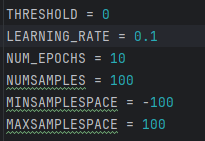
\includegraphics[scale=0.75]{../figs/P1.1.png}\\
\end{center}

\begin{center}
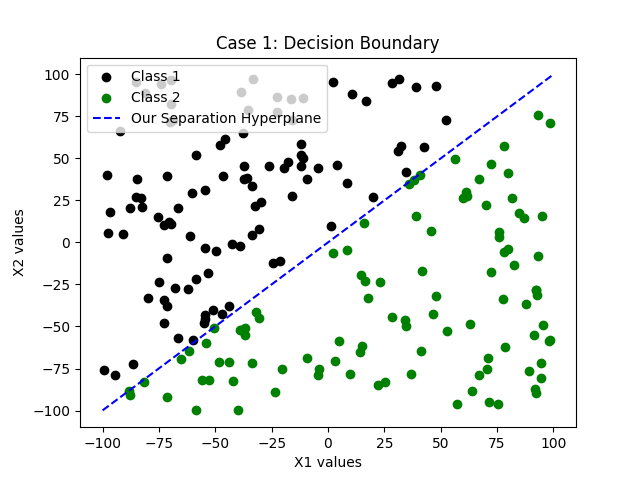
\includegraphics[scale=0.75]{../figs/P1.2.png}\\
\end{center}

\begin{center}
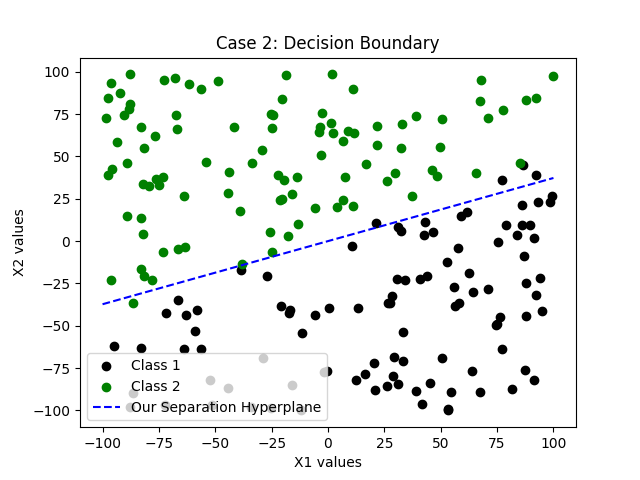
\includegraphics[scale=0.75]{../figs/P1.3.png}\\
\end{center}

\begin{center}
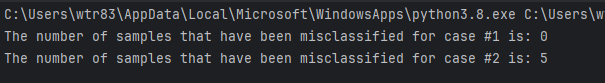
\includegraphics[scale=0.75]{../figs/P1.4.png}\\
\end{center}

\subsection{1,000 Samples}

For our additional test with 1,000 samples...

\begin{center}
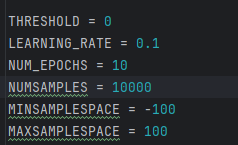
\includegraphics[scale=0.75]{../figs/P2.1.png}\\
\end{center}

\begin{center}
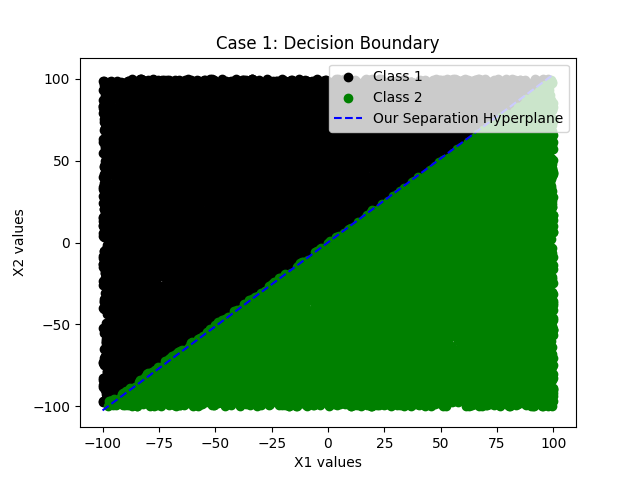
\includegraphics[scale=0.75]{../figs/P2.2.png}\\
\end{center}

\begin{center}
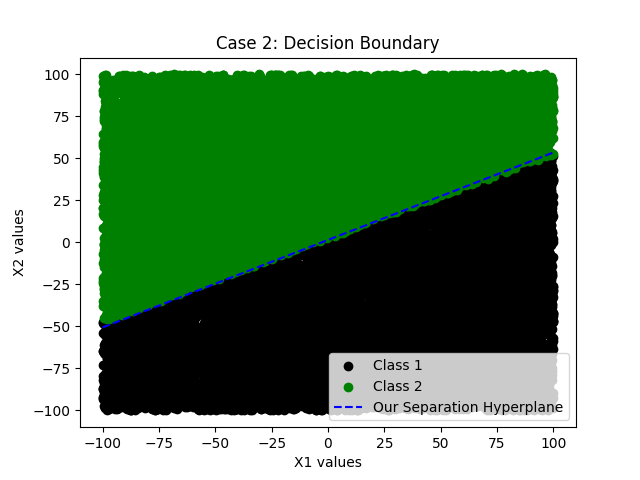
\includegraphics[scale=0.75]{../figs/P2.3.png}\\
\end{center}

\begin{center}
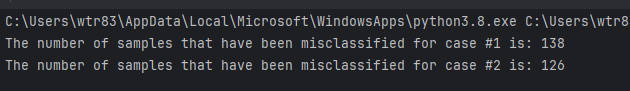
\includegraphics[scale=0.75]{../figs/P2.4.png}\\
\end{center}

\section{Gradient Descent}

For parts 4-5 of the assignment... (general overview).

\subsection{Standard Test}

Talk about initial test.

\subsection{Additional Test}

Talk about additional test and observations.

\end{document}
